\chapter{Testing and Validation}
\setlength{\parindent}{0pt}
\setlength{\parskip}{6pt}
{\setstretch{1.5}

This chapter presents the testing and validation of the \textbf{ResQNow} emergency response system. The objective of this phase is to verify that all functional modules operate correctly, meet performance requirements, and remain reliable under real-world conditions. System behavior is validated through structured testing procedures, quantitative performance measurements, and graphical analysis of observed results.

% -----------------------------------------------------------------------------
\section{Objective of Testing}

The primary objective of testing ResQNow is to ensure correctness, reliability, and robustness of all integrated modules. The testing phase aims to:
\begin{itemize}
    \item Verify correct functioning of SOS activation and alert delivery mechanisms.
    \item Validate AI-based emergency classification accuracy.
    \item Measure responsiveness of AR-based first-aid guidance.
    \item Evaluate BLE-based offline communication reliability.
    \item Ensure system stability under varying network conditions.
\end{itemize}

% -----------------------------------------------------------------------------
\section{Test Environment}

All tests were conducted on real mobile devices under both controlled and real-world operating conditions. Table~\ref{tab:test_environment} summarizes the hardware and software environment used for testing. The selected environment closely resembles real emergency situations by considering variations in device capabilities, operating systems, and network availability. Testing was performed across multiple connectivity modes including Wi-Fi, mobile data, and offline BLE scenarios to evaluate system robustness. This ensured that the ResQNow system maintained consistent performance, reliability, and responsiveness during practical emergency usage conditions.


\begin{table}[H]
\centering
\caption{Test Environment Configuration}
\label{tab:test_environment}
\begin{tabular}{|p{5cm}|p{8cm}|}
\hline
\textbf{Component} & \textbf{Specification} \\ \hline
Mobile Platforms & Android 13, iOS 17 \\ \hline
Development Framework & Flutter (v3.x) \\ \hline
Backend Services & Python (FastAPI), Firebase Cloud Functions \\ \hline
Database & Firebase Firestore \\ \hline
AR Framework & ARCore SDK \\ \hline
AI Services & Cloud-based conversational AI APIs \\ \hline
Connectivity Modes & Wi-Fi, 4G, Offline (BLE) \\ \hline
Test Devices & Pixel 6, OnePlus 9, iPhone 12 \\ \hline
\end{tabular}
\end{table}

% -----------------------------------------------------------------------------

\section{System Testing Approach}

The ResQNow emergency response system was validated using a comprehensive testing methodology to ensure functional correctness, seamless integration, system reliability, and acceptable performance under different operating conditions. Multiple testing strategies were applied to evaluate both individual components and the fully integrated system.

Initially, unit testing was performed to verify the correctness of core modules such as SOS activation, GPS location capture, BLE-based communication, AI-driven emergency classification, and notification handling. Each module was tested independently using predefined inputs to identify functional errors at an early stage of development.

Following this, integration testing was conducted to validate interactions between the mobile application, backend services, AI modules, and notification systems. This phase ensured proper data exchange, API communication, and synchronization across system layers.

System testing involved end-to-end validation of the complete emergency workflow, from SOS initiation through alert dissemination and AR-based first-aid guidance. This confirmed that all components functioned cohesively to meet system requirements.

Finally, performance testing evaluated system responsiveness, latency, and resource usage under varying network conditions. Key metrics such as SOS dispatch time, AI response delay, AR initialization time, and BLE relay latency were measured to assess real-time operational efficiency.


% -----------------------------------------------------------------------------
\section{Functional Test Case Validation}

Key functional test cases were executed to validate expected system behavior across different usage scenarios. Table~\ref{tab:functional_tests} presents representative test cases and their outcomes. The test cases were designed to cover critical user actions, system responses, and failure-handling conditions to ensure functional completeness. Successful execution of these cases confirms that core features operate reliably under normal and edge-case scenarios. Additionally, the validation process ensured that error conditions were handled gracefully without affecting overall system stability. These results demonstrate that the functional requirements of the ResQNow system are fully satisfied.

\begin{table}[H]
\centering
\caption{Functional Test Cases and Validation Results}
\label{tab:functional_tests}
\begin{tabular}{|p{1cm}|p{5cm}|p{5cm}|p{2cm}|}
\hline
\textbf{No.} & \textbf{Test Case} & \textbf{Expected Outcome} & \textbf{Result} \\ \hline
1 & User Registration & Account created successfully & Pass \\ \hline
2 & SOS Activation & Alert sent within 2 seconds & Pass \\ \hline
3 & AI Classification & Correct severity detected & Pass \\ \hline
4 & AR Guidance Launch & AR overlay loads correctly & Pass \\ \hline
5 & Push Notification & Contacts notified & Pass \\ \hline
6 & BLE Offline Relay & SOS relayed successfully & Pass \\ \hline
7 & Location Tracking & Continuous GPS updates & Pass \\ \hline
\end{tabular}
\end{table}

% -----------------------------------------------------------------------------
\section{Performance Validation Results}
Quantitative performance metrics were collected during testing, and Table~\ref{tab:performance_validation} summarizes the measured results indicating that the system meets requirements under real-time emergency operating conditions.

\begin{table}[H]
\centering
\caption{Performance Validation Metrics}
\label{tab:performance_validation}
\begin{tabular}{|p{4cm}|p{4cm}|p{4cm}|p{2cm}|}
\hline
\textbf{Module} & \textbf{Metric} & \textbf{Observed Value} & \textbf{Status} \\ \hline
SOS Dispatch & App to backend latency & 1.8 seconds & Validated \\ \hline
AI Classification & Response time & 2.3 seconds & Validated \\ \hline
AR Module & Initialization latency & 1.2 seconds & Validated \\ \hline
BLE Relay & Offline forwarding delay & 6.5 seconds & Validated \\ \hline
Battery Usage & 1 hour usage & 9\% drain & Acceptable \\ \hline
\end{tabular}
\end{table}

To visualize the relative latency of major system modules, a comparative bar chart is shown in Figure~\ref{fig:latency_graph}. The chart enables easy comparison of response times across different modules under identical testing conditions.


\begin{figure}[H]
\centering
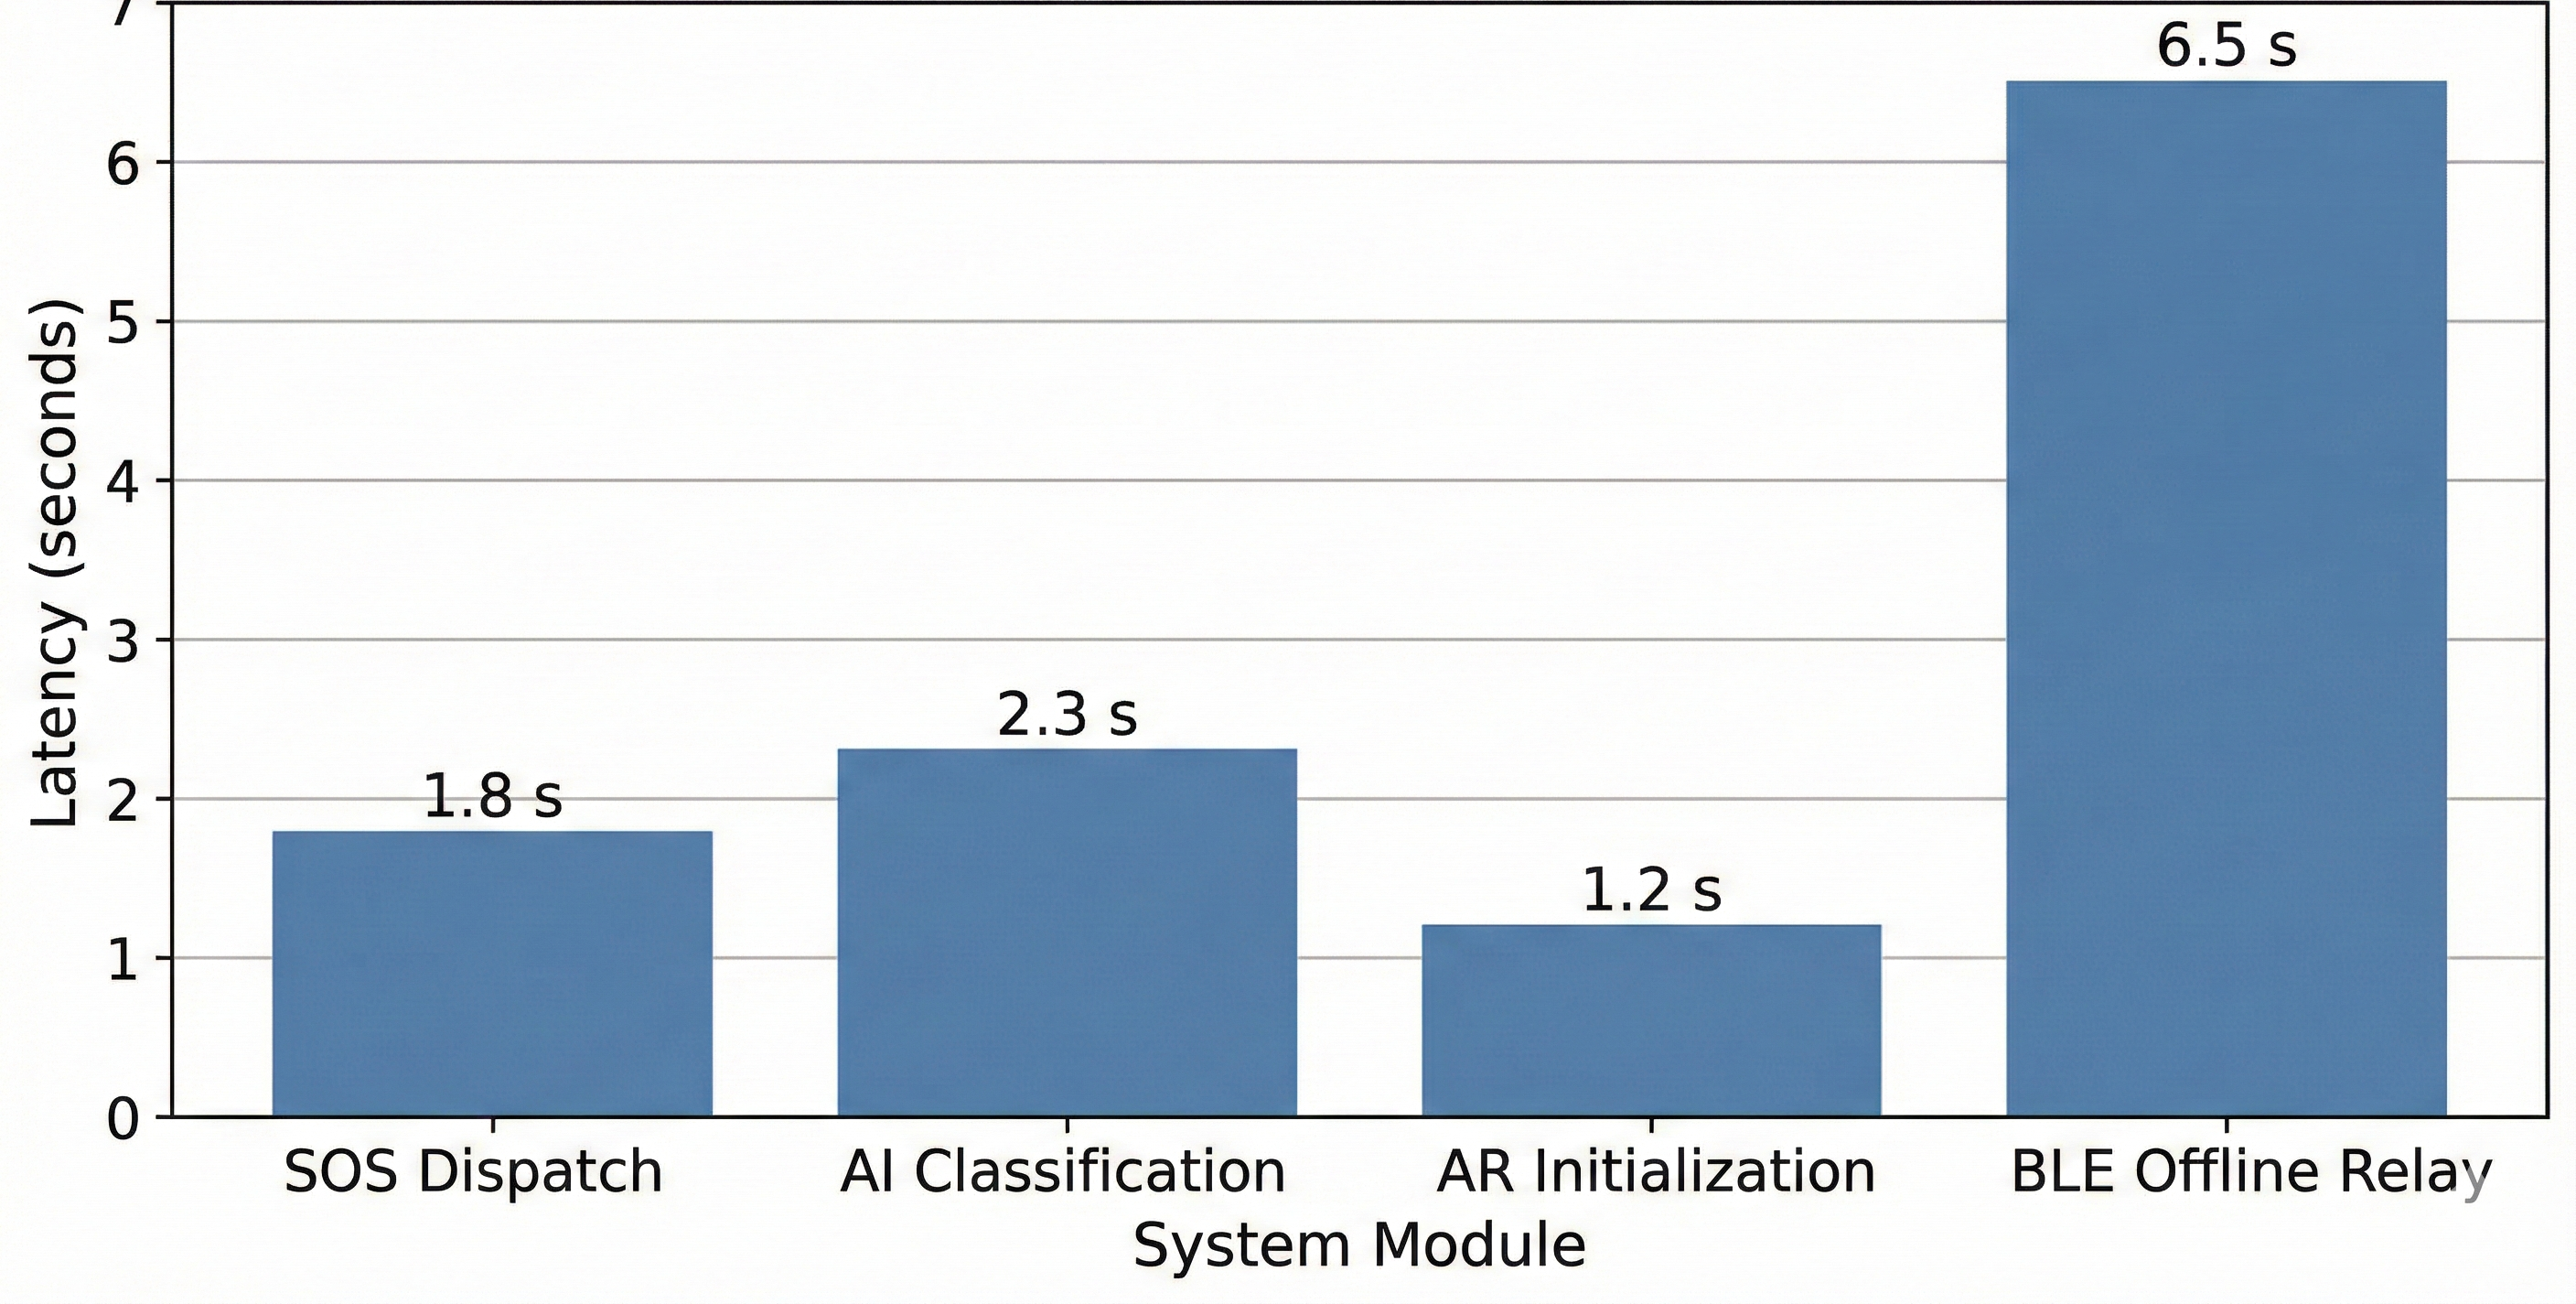
\includegraphics[width=\textwidth]{chapters/latency_comparison.png}
\caption{Comparison of latency across SOS, AI classification, AR initialization, and BLE relay}
\label{fig:latency_graph}
\end{figure}

% -----------------------------------------------------------------------------
\section{Offline Communication Validation}

BLE-based offline SOS relay reliability was evaluated at varying hop counts and distances. Table~\ref{tab:ble_validation} presents the measured success rates. The evaluation focuses on assessing the effectiveness of BLE-based peer-to-peer communication in the absence of internet connectivity. The results help determine the feasibility of offline SOS message propagation in emergency scenarios.

\begin{table}[H]
\centering
\caption{BLE-Based Offline Communication Validation}
\label{tab:ble_validation}
\begin{tabular}{|p{4cm}|p{4cm}|p{3cm}|}
\hline
\textbf{Relay Scenario} & \textbf{Distance} & \textbf{Success Rate (\%)} \\ \hline
Single-hop & 5 meters & 96 \\ \hline
Two-hop & 10 meters & 92 \\ \hline
Three-hop & 15 meters & 88 \\ \hline
\end{tabular}
\end{table}

Figure~\ref{fig:ble_graph} compares the latency characteristics of SOS delivery, AI classification, AR initialization, and BLE-based communication. The comparison highlights that BLE relay introduces higher delay compared to online modules, yet remains within acceptable limits for offline emergency message forwarding.

\begin{figure}[H]
\centering
\includegraphics[width=\textwidth]{chapters/ble_success_rate.png}
\caption{BLE offline relay success rate versus hop count}
\label{fig:ble_graph}
\end{figure}

% -----------------------------------------------------------------------------
\section{AI Classification Validation}

The AI-based emergency classification module of the ResQNow system was validated to assess its accuracy across different emergency scenarios. Test inputs representing emergencies such as cardiac arrest, bleeding, fractures, burns, and respiratory distress were provided to the system. The AI model successfully analyzed user-described symptoms and classified emergencies into appropriate categories with corresponding severity levels. High accuracy was observed for critical emergencies, enabling effective prioritization and alert dispatch. The inclusion of contextual information improved classification reliability by reducing ambiguity in user input. These results demonstrate that the AI module can effectively support intelligent triage during real-world emergency situations.

\begin{figure}[H]
\centering
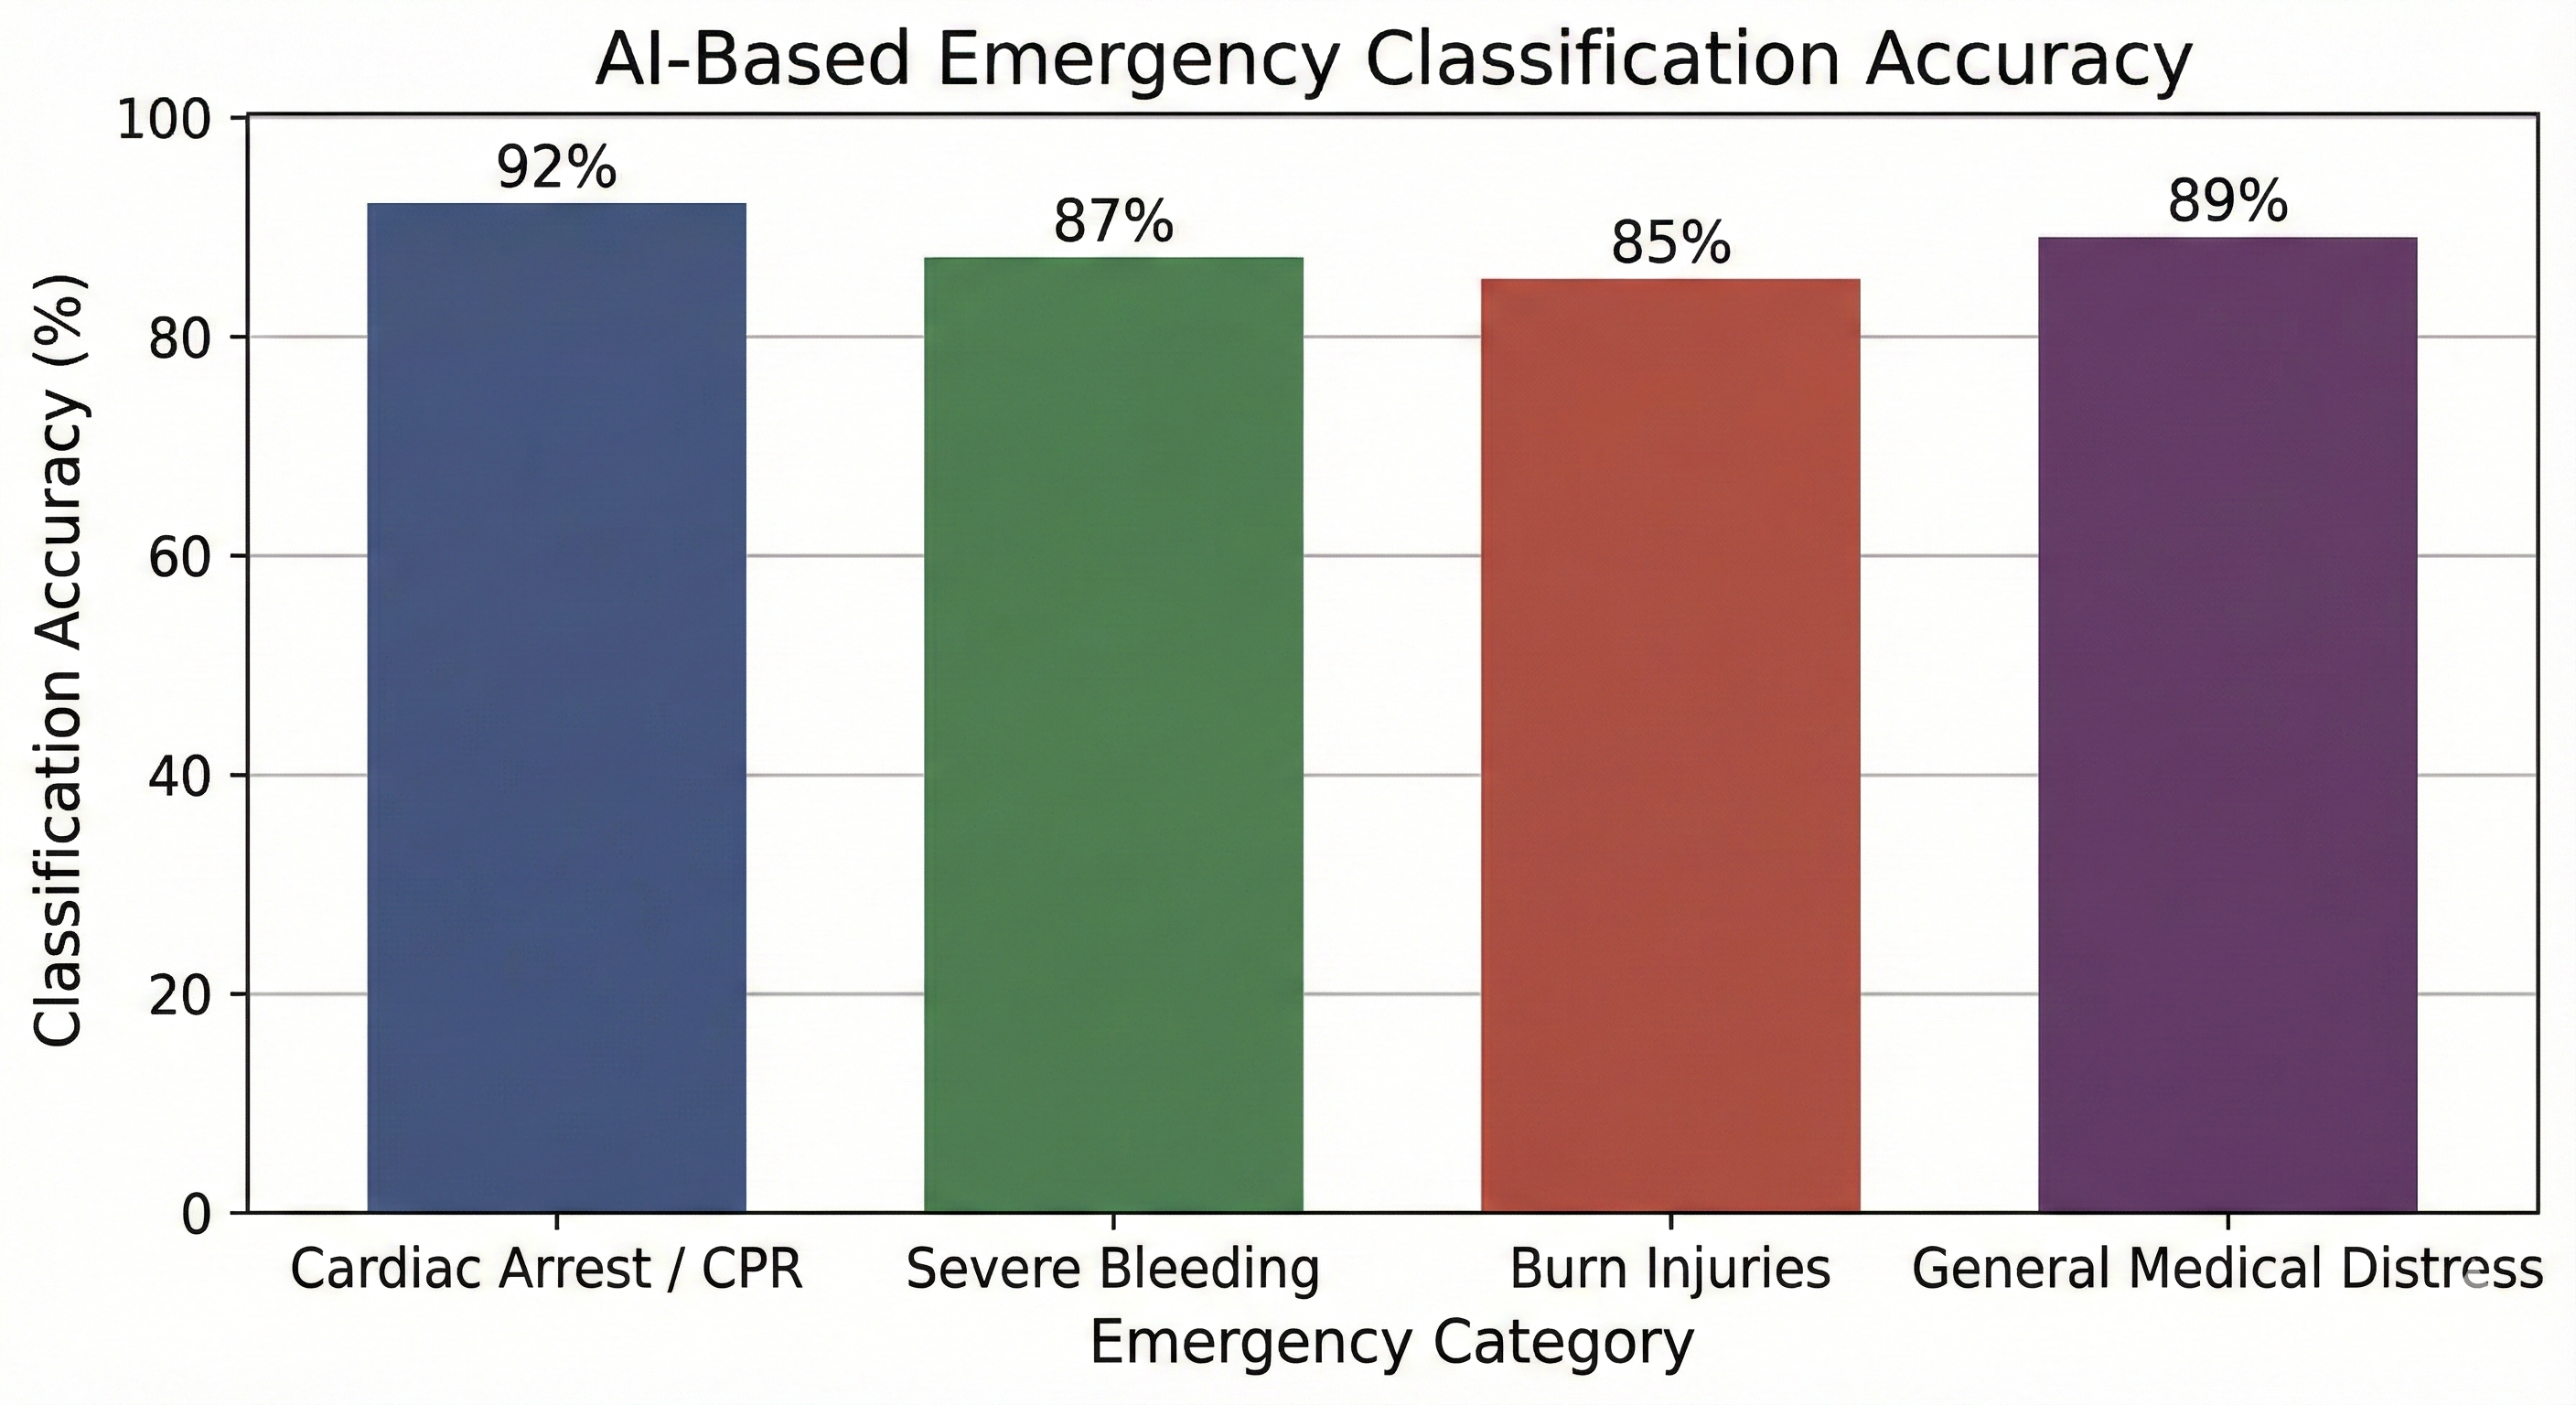
\includegraphics[width=\textwidth]{chapters/ai_accuracy.png}
\caption{AI-based emergency classification accuracy across different emergency categories}
\label{fig:ai_accuracy}
\end{figure}

% ---------------------------------------------------------------------------
}
